\hypertarget{ux5f00ux53d1ux652fux6301}{%
\chapter{开发支持工具}\label{ux5f00ux53d1ux652fux6301}}

在疫情期间,由于团队成员异地协作难度较高,经由指导老师的支持,我们完成了如下系统的构建。提升了协作效率。

\hypertarget{ux81eaux52a8ux5316ux6784ux5efaux53caux6d4bux8bd5}{%
\section{自动化构建及测试}\label{ux81eaux52a8ux5316ux6784ux5efaux53caux6d4bux8bd5}}

得益于周老师提供的一台10核32G内存150G硬盘的服务器,及北邮人团队的校内Git服务器,参考并重写清华Nontrival-mips提供的自动构建脚本,通过在服务器上对\texttt{vivado}进行\texttt{docker}封装,我们成功建立校园环境内的自动构建服务器。
该服务器可以完成如下功能:

\begin{enumerate}
\item
  自动完成功能、性能、TLB测试的Simulation阶段
\item
  自动完成\texttt{func/perf\ bitstream}的构建,并上传到平台以供下载。
\item
  提供时序检查报告的下载。
\end{enumerate}

通过该自动构建服务器,帮助我们解决了远程协作时代码的有效性问题,减少了merge分支时带来的出错可能。

\begin{figure}[ht]
    \centering
    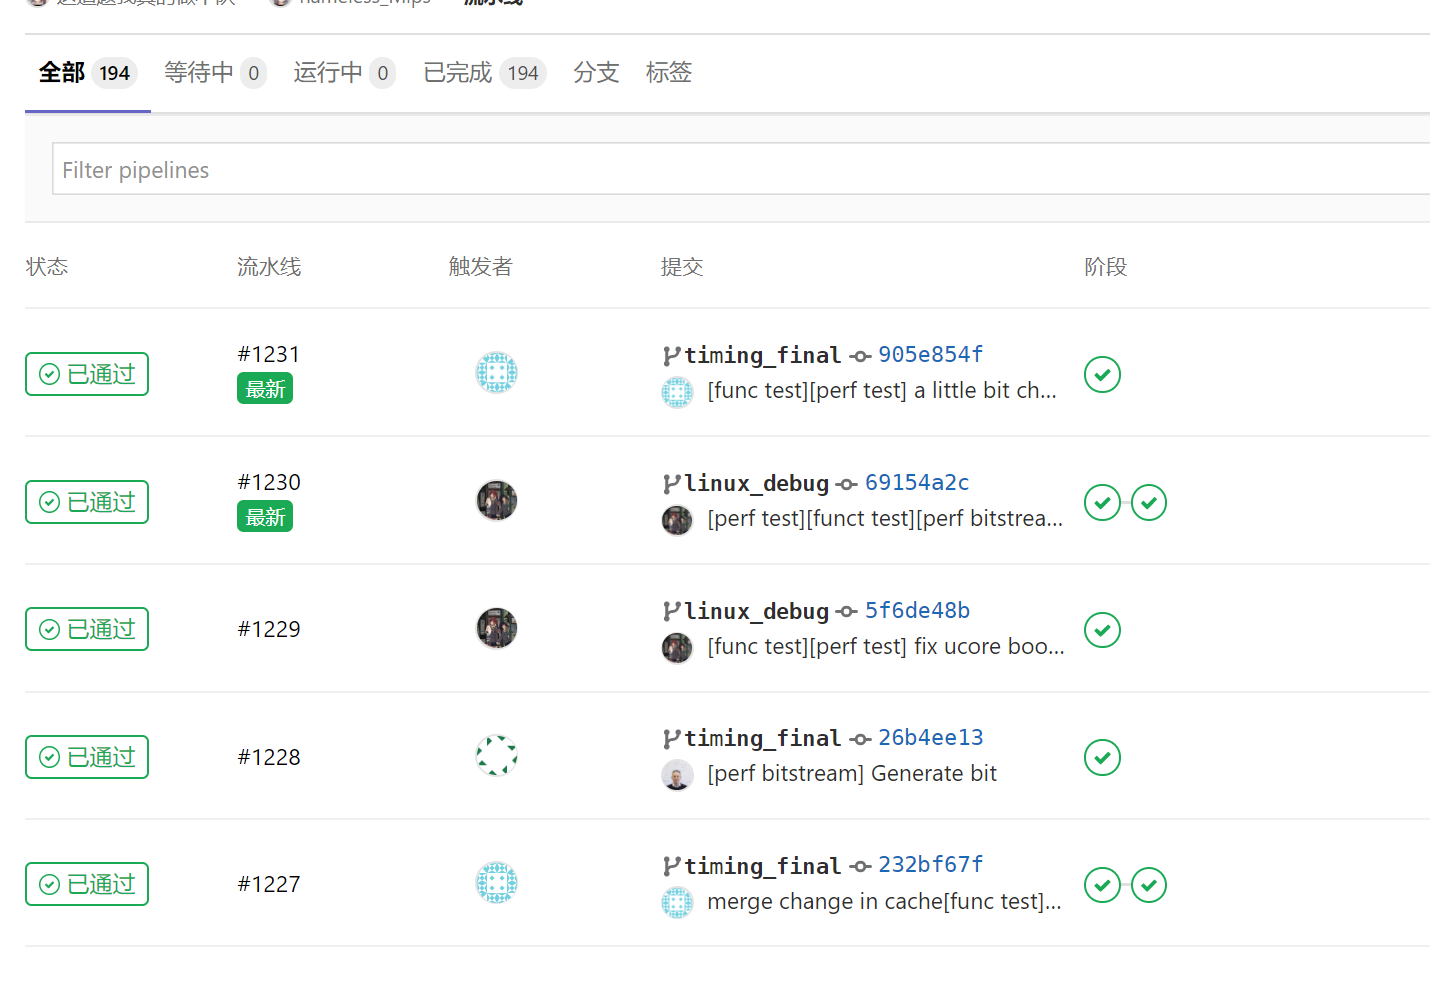
\includegraphics[width=0.7\linewidth]{ci_usage.png}
    \caption{CI使用情况}
    \label{fig:ci-usage}
\end{figure}

\hypertarget{ux75abux60c5ux671fux95f4ux8fdcux7a0bux534fux4f5c}{%
\section{疫情期间远程协作}\label{ux75abux60c5ux671fux95f4ux8fdcux7a0bux534fux4f5c}}

在疫情期间,团队协作问题给我们的进展带来了很大的困扰。同时团队成员的电脑性能不足也令开发进度受到限制,运行测试时时间长和复现问题困难;还因为系统测试板仅有一块,在执行后续调试时问题较为繁多。
为此,我们通过如下两种方法解决:

\begin{enumerate}
\item
  通过在校内服务器上进行内网穿透并配置\texttt{VNC}远程桌面,进行远程编写。解决本地计算机性能不足和环境不同(macOS)的问题,节省调试时间并给本地留出更多的性能。
\item
  通过Teamviewer进行远程桌面,在调试系统测试的波形问题时,不需要频繁上传下载波形即完成。配合语音通话并进行同屏协作,调试效率大大提升,比单纯靠语音描述更加有效。
\end{enumerate}

整个开发过程中,我们一共进行了270余次提交,完成了194次有效的自动化构建,节省的总时长大约为230小时。

在穿透时,我们选择仅支持\texttt{ssh\_public\_key},设置不常用用户名来避免暴力破解,按需开启VNC功能,在方便了自身的同时确保校内网络安全。
